\section{Gateway IoT}
\label{sec:iotGateway}

Ao utilizar IoT, de imediato temos algo que estará conectado à Internet. Esse \textit{"algo"} não necessariamente se conecta de forma direta. Na grande maioria dos casos, essa conexão se dá por meio um gateway. Gateway IoT é uma aplicação (ou dispositivo com aplicação embarcada) responsável por receber requisições de diversos sensores e em algumas situações executar ações \cite{ChenJiaLi}. 

O gateway é similar a um roteador \footnote{Roteador é um dispositivo físico de rede cujo objetivo é encaminhar pacotes entre redes de computadores}, porém, ele pode unir redes de diferentes protocolos através de um processamento local para a tradução e conversão de protocolos. Gateways são muito utilizados em ambiente industrial e corporativo, porém, com o avanço da IoT, é mais comum encontrar esse tipo de equipamento para uso residencial.

Com a evolução dos gateways são utilizados basicamente dois tipos de Gateways IoT \cite{WhatIsIotGateway}, os \textit{Traditional Gateways} que não são inteligentes e apenas armazenam a informações para futura transmissão, e os \textit{Smart Gateways} que além disso, podem fazer ações, tais como:
\begin{itemize}
	\item Persistir as informações;
	\item Efetuar transformação dos dados recebidos;
	\item Guardar os dados temporariamente para posteriormente transmiti-los para a Internet;
	\item Executar regras de segurança sobre os dispositivos;
	\item Executar ações com base nos dados recebidos e regras configuradas.
\end{itemize}

A Figura \ref{fig:arquiteturaIotGateway} ilustra uma arquitetura convencional de um Gateway IoT e suas relações com os sensores e com a Cloud.
\begin{figure}[h!]
	\begin{center}
		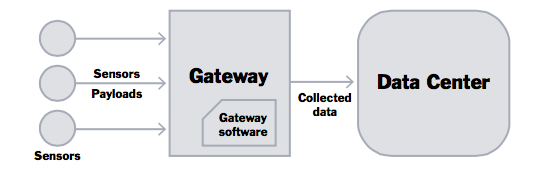
\includegraphics[width=1\textwidth]{./img/rumFxS7.png}
		\caption{Descrição esquemática da arquitetura de um Gateway IoT. \cite{DZone}}
		\label{fig:arquiteturaIotGateway}
	\end{center}
\end{figure}

Sensores residem no que a indústria nomeia como sendo campo, ou seja, onde os sensores realmente devem atuar. São exemplos de campos: galpões, silos, plantas industriais, florestas, plantações etc. Já a Cloud tem o mesmo significado que estamos habituados: um servidor na nuvem onde dados são mantidos e processamentos são realizados. O Gateway IoT faz exatamente essa ligação entre os sensores e a Internet, uma vez que sensores não costumam ter boas condições de acesso à Internet, tanto do ponto de vista da disponibilidade quanto da largura de banda.

A grande vantagem em construir um Gateway open-source é o alto nível de customização que ele pode oferecer, já que temos total acesso ao sistema operacional, sem restrições impostas pelo fabricante – o que ocorre na maioria dos casos. Essa customização vai permitir usar o gateway em modo \textit{fog computing} \footnote{\textit{Fog Computing}, ou Computação em Névoa, define a arquitetura que estende a capacidade computacional e o armazenamento da nuvem para as camadas de acesso da rede, permitindo que os dados sejam analisados e transformados em informações ou em ações antes de serem simplesmente transmitidos. \cite{CIOIDG}} para o processamento de informações o mais perto do dispositivo da borda, ou \textit{edge device}, fazendo com que, mesmo na falta de Internet, o dispositivo consiga se manter operacional, ainda que com algumas restrições.

Fazer o seu próprio gateway de IoT pode parecer contra-intuitivo à primeira vista, mas com a baixa nos preços dos SoC’s (System-on-a-Chip) \footnote{\textit{System-on-a-chip}, ou simplesmente \textit{SoC}, é um termo utilizado para caracterizar um circuito integrado que engloba todos os componentes de um computador convencional, tais como CPU, GPU (processador gráfico), memória RAM, módulo Wi-Fi, interfaces externas etc. O Raspberry Pi é um dos mais populares exemplares de \textit{SoC}}, alavancado principalmente pela Raspberry Pi \cite{RaspberryPi}, torna possível a criação de sistemas computacionais de bom desempenho, tamanho reduzido e baixo custo. Já é possível encontrar SoC’s custando menos de US\$ 10 e chips completos e funcionais por menos de US\$ 40 \cite{RaspberryPiVenda}.